% !TeX spellcheck = <none>
\documentclass[a4paper, 10pt]{article}

%\usepackage{cmap}
\usepackage[T2A]{fontenc}
\usepackage[utf8]{inputenc}
\usepackage[english, russian]{babel}
\usepackage{graphicx}
\usepackage[top=2cm, bottom=2cm, left=3cm, right=2cm]{geometry}
\graphicspath{./}
\usepackage{biblatex}
\addbibresource{lib.bib}
\linespread{1.5}
{\usefont{T2A}{Tempora-TLF}{m}{n}
\usepackage{amsmath}

\usepackage{ragged2e}
\justifying

\usepackage{listings}
\usepackage{color}


\definecolor{codegreen}{rgb}{0,0.6,0}
\definecolor{codegray}{rgb}{0.5,0.5,0.5}
\definecolor{codepurple}{rgb}{0.58,0,0.82}
\definecolor{backcolour}{rgb}{0.95,0.95,0.92}

\lstdefinestyle{mystyle}{
	backgroundcolor=\color{backcolour},   
	commentstyle=\color{codegreen},
	keywordstyle=\color{magenta},
	numberstyle=\tiny\color{codegray},
	stringstyle=\color{codepurple},
	basicstyle=\ttfamily\footnotesize,
	breakatwhitespace=false,         
	breaklines=false,                 
	captionpos=b,                    
	keepspaces=true,                 
	numbers=left,                    
	numbersep=5pt,                  
	showspaces=false,                
	showstringspaces=false,
	showtabs=false,                  
	tabsize=4
}

\lstset{style=mystyle}

\begin{document}
	
\begin{titlepage}
	\fontsize{12pt}{12pt}\selectfont
	\begin{figure}[t!]
		\centering
		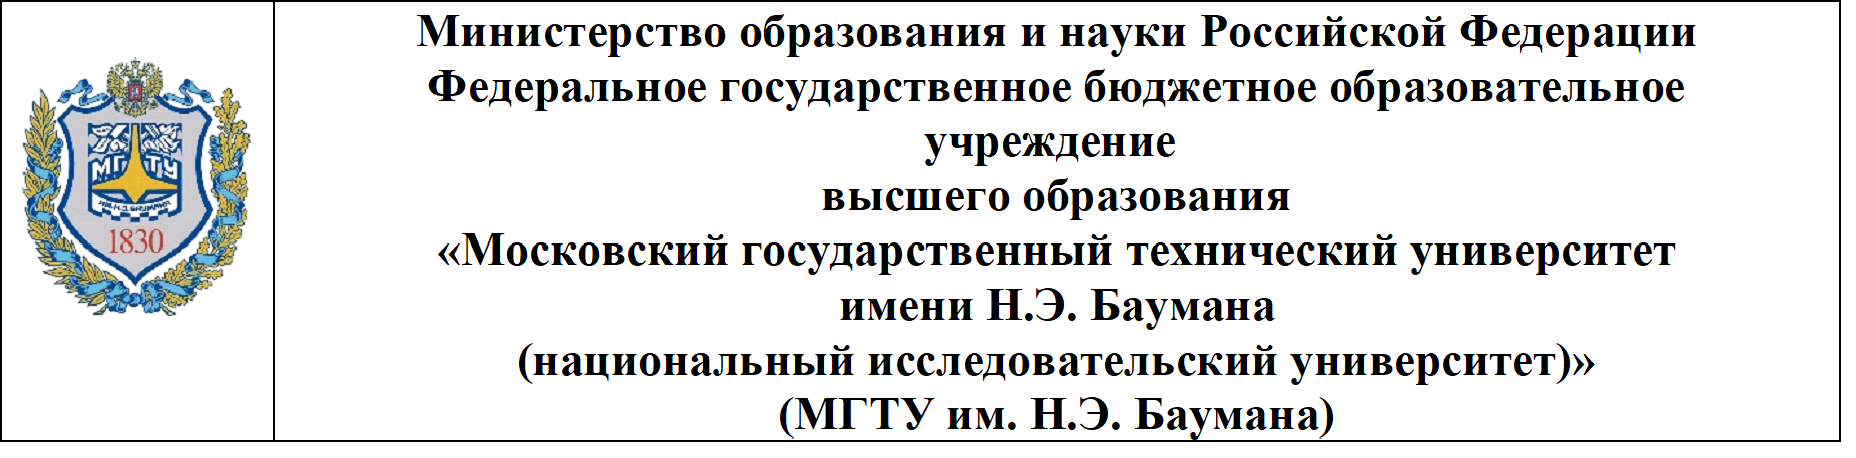
\includegraphics[scale=0.8]{bmstu}
	\end{figure}
	
	\noindent\rule{15cm}{3pt}
	\newline\newline
	\noindent 
	ФАКУЛЬТЕТ 
	\underline{«Информатика и системы управления»} \newline
	
	\noindent КАФЕДРА \underline{«Программное обеспечение ЭВМ и информационные технологии»}\newline\newline\newline\newline\newline
	
	\centering {\Large \textbf{\hspace*{1cm}РАСЧЕТНО-ПОЯСНИТЕЛЬНАЯ ЗАПИСКА}} 
	\newline \\ \centering{\Large \textbf{\textit{\hspace*{20mm}К КУРСОВОЙ РАБОТЕ}}}
	\newline \\ \centering{\Large \textbf{\textit{НА ТЕМУ:}}}
	\vspace{3mm}
	
	\centering{\LARGE \textrm{<<Загружаемый модуль ядра для защиты персональных данных>>}
		\vspace{10mm}	
		
	\vspace{10mm}}

	\begin{flushleft}
		Студент
		$\underset{\text{  (Группа)}}{\hspace{0.6cm}\underline{\hspace{0.6cm}\text{ИУ7-76Б}\hspace{0.6cm}}}$
		\hspace{30mm}$\underset{\text{(Подипсь, дата)}}{\underline{\hspace{4cm}}}$ 
		\hspace{4mm}$\underset{\text{(И.О.Фамилия)}}{\underline{\text{Ж.Р.Турсунов}}}$ 
	\end{flushleft}

	\begin{flushleft}
		Руководитель курсового проекта
		\hspace{2cm}$\underset{\text{(Подипсь, дата)}}{\underline{\hspace{4cm}}}$ 
		\hspace{4mm}$\underset{\text{(И.О.Фамилия)}}{\underline{\text{Н.Ю.Рязанова}}}$ 
	\end{flushleft} 

	\begin{flushleft}
		Консультант
		\hspace{5.8cm}$\underset{\text{(Подипсь, дата)}}{\underline{\hspace{4cm}}}$ 
		\hspace{4mm}$\underset{\text{(И.О.Фамилия)}}{\underline{\hspace*{3cm}}}$ 
	\end{flushleft}    
	
	\begin{center}
		\vfill
		Москва, \the\year
		~г.
	\end{center}
	\clearpage
	\newpage
	\begin{center}
		\centering{\hspace{10mm} \small \bf Министерство науки и высшего образования Российской Федерации
			Федеральное государственное бюджетное образовательное учреждение
			высшего образования \\ <<Московский государственный технический университет имени Н.Э.Баумана\\(национальный исследовательский университет)>>\\(МГТУ им. Н.Э.Баумана)} 
		\noindent\rule{\textwidth}{2pt}
	\end{center}
	\begin{flushright}
		\normalsize{УТВЕРЖДАЮ \\
			Заведующий кафедрой$\underset{\text{(Индекс)}}{\underline{\text{ИУ7}}}$ 
			\\ \vspace{1mm} $\underset{}{\underline{\hspace{3cm}}}$ \hspace{2mm}$\underset{\text{(И.О.Фамилия)}}{\underline{\text{И.В.Рудаков}}}$
			\\ \vspace{1mm}<<$\underset{}{\underline{\hspace{0.7cm}}}$ >> $\underset{}{\underline{\hspace{3cm}}}$2021 г.} 
	\end{flushright}
	
	\begin{center}
		\large{\bf{ЗАДАНИЕ
				\\ на выполнение курсовой работы}}
	\end{center}
	\begin{flushleft}
		\normalsize{по дисциплене $\underset{}{\underline{\hspace*{1cm} \text{Операционные системы} \hspace*{87mm}}}$
			\\Студент группы \underline{\hspace{1cm} \text{ИУ7-76Б} \hspace{1cm}}
			\\ $\underset{ \text{(Фамилия, имя, отчество)}}{\underline{\hspace*{6cm} \text{Турсунов Жасурбек Рустамович} \hspace*{47mm}}}$
			\\Тема курсовой работы \underline{\text{\hspace{1mm} Загружаемый модуль ядра защиты персональных данных \hspace*{9mm}}}
			\\ Направленность КР (учебная, исследовательская, практическая, производственная, др.)
			\\ \underline{\hspace{6cm} \text{учебная} \hspace{85mm}}
			\\ Источник тематики (кафедра, предприятие, НИР)\underline{\hspace{2cm} \text{кафедра} \hspace{42mm}}
			\\График выполнения проекта:  25\% к \underline{\hspace*{0.5cm}} нед., 50\% к \underline{\hspace*{0.5cm}} нед., 75\% к \underline{\hspace*{0.5cm}} нед., 100\% к \underline{\hspace*{0.5cm}} нед.}
	\end{flushleft}
	\normalsize {{ \textbf{\textit{Задание}}} \underline{Необходимо реализовать загружаемый модуль ядра для отслеживания изменений в USB-\hspace*{1mm}} \\ \underline{портах и проверки на наличие доступа к секретным файлам. В случае отстутствия допуска - зашиф- } \\ \underline{ровать все запрещенные для копирования файлы.\hspace*{8cm}}}
	\\ \normalsize {{\textbf{\textit{Оформление курсовой работы:}}}}
	\\ Расчетно-пояснительная записка на \underline{20-30} листах формата А4.
	
	\underline{Расчетно-пояснительная записка должна содержать введение, аналитическую часть, конструк-} \\ \underline{торскую часть, технологическую часть, экспериментально-исследовательский раздел, заключение,} \\ \underline{список литературы, приложения. \hspace*{10.5cm}}
	
	\begin{flushleft}
		\small Дата выдачи задания <<\underline{\hspace{1cm}}>> \underline{\hspace{3cm}} 2021 г.
		\newline
		\\ \small \textbf{Руководитель курсового проекта}
		\small \hspace{3cm}$\underset{\text{(Подипсь, дата)}}{\underline{\hspace{4cm}}}$ 
		\small \hspace{4mm}$\underset{\text{(И.О.Фамилия)}}{\underline{\text{Н.Ю.Рязанова}}}$ 
	\end{flushleft}
	\begin{flushleft}
		\small \textbf{Студент}
		\small \hspace{7.2cm}$\underset{\text{(Подипсь, дата)}}{\underline{\hspace{4cm}}}$ 
		\small \hspace{5mm}$\underset{\text{(И.О.Фамилия)}}{\underline{\text{Ж.Р.Турсунов}}}$ 
	\end{flushleft}
	
\end{titlepage}
\setcounter{page}{3}
\tableofcontents
\clearpage
\newpage


\section*{Введение}
\addcontentsline{toc}{section}{Введение}

\hspace*{5mm} В настоящее время одним из способов защиты персональных данных на компьютере, является защита доступа к данным путем идентификации пользователя с использованием USB-устройства. Однако данный способ в силу его распрастраненности не является надежным, так как существуют специальные USB флеш-памяти с наиболее часто используемыми идентификаторами производителя и самого устройства.

Данная работа посвящена к разработке программного обеспечения для защиты данных на компьютере с использованием флеш-памяти с дополнительными средствами защиты информации.

	
\clearpage
\newpage
\section{Аналитический раздел}
	\subsection{Постановка задачи}
	\hspace*{5mm} В соответствии с заданием на курсовую работу необходимо разработать программное обеспечение для защиты персональных данных. Для решения поставленной задачи необходимо:
	\begin{enumerate}
		\item проанализировать способы защиты при помощи USB флеш-памяти;
		\item определить основные понятия;
		\item разработать алгоритм;
		\item реализовать загружаемый модуль ядра.
	\end{enumerate}
	\hspace*{5mm} На вход подается USB-устройство с паролем. На выходе получаем зашифрованый или расшифрованный файл.
	
	\subsection{Загружаемый модуль ядра}
	\hspace*{5mm} Ядро Linux динамически изменяемое -- это означает, что вы можете загружать в ядро дополнительную функциональность, выгружать функции из ядра и даже добавлять новые модули, использующие другие модули ядра. Преимущество загружаемых модулей заключается в возможности сократить расход памяти для ядра, загружая только необходимые модули (это может оказаться важным для встроенных систем).
	
	Загружаемый модуль представляет собой специальный объектный файл в формате ELF (Executable and Linkable Format). Для работы с загружаемыми модулями можно использовать стандартные средства работы с объектными файлами (имеют суффикс .ko, от kernel object) [2].
	
	
	В OC Linux существуют специальные команды для работы с загружаемыми модулями ядра:
	\begin{enumerate}
		\item insmod -- Загружает модуль в ядро из конкретного файла, если модуль зависит от других модулей. Только суперпользователь может загрузить модуль в ядро;
		\item lsmod -- Выводит список модулей, загруженных в ядро;
		\item modinfo -- Извлекает информацию из модулей ядра (лицензия, автор, описание);
		\item rmmod -- Команда используется для выгрузки модуля из ядра, в качестве параметра передается имя файла модуля. Только суперпользователь может выгрузить модуль из ядра.
	\end{enumerate}
	
	Загружаемые модули ядра должны содержать два макроса module\_init и module\_exit.
	
	\subsection{Адресное пространство  USB-устройств}
	\hspace*{5mm}Каждое внешнее запоминающее устройство имеет в descriptor Vendor ID и Product ID. Регистры Vendor ID и Device ID идентифицируют устройство. Шестнадцатиразрядный регистр Vendor ID выдаётся организацией PCI SIG. Шестнадцатиразрядный регистр Device ID назначается изготовителем устройства.
	
	Для того, чтобы обращаться к устройству через адресное пространство памяти или ввода-вывода, системное программное обеспечение или ОС программирует базовые адресные регистры (англ. Base Address Registers, также называемые BAR’ами), посылая конфигурационные команды USB-контроллеру. В начале загрузки системы все USB устройства находятся в неактивном состоянии, им не назначены адреса, по которым драйверы устройств могут взаимодействовать с ними. Либо BIOS, либо сама операционная система обращается к USB слотам и настраивает BAR’ы в конфигурационном адресном пространстве. Значения BAR’ов действительны всё время, пока система включена. При отключении питания значения этих регистров теряются до следующей загрузки, в процессе которой процедура настройки повторяется. Так как этот процесс полностью автоматизирован, пользователь компьютера освобождается от непростой задачи конфигурирования нового аппаратного обеспечения, подключаемого к шине USB.
	

	В данной работе поисходит отслеживание изменений на USB-портах, основными используемыми структурами являются usb\_device и usb\_device\_id. B структуры представлены в листингах 3 и 4 соответственно.
	\subsection{Хранение информации о доступных USB-устройствах}
	Так как в USB-порты могут подключаться любые устройства типа USB, необходимо создать список устройств разрешенных для подключения и доступа к секретным файлам. Для распознания устройства при его подключении к USB-порту необходимо сканировать весь список зарегестрированых и существующих в системе устройств которые хранятся в виде двусвязного списока ядраа Linux, реализованный в файле \#include/linux/list.h [5] и определить входит ли он в список разрешенных устройств. Ниже предаствлены основные функции для сканирования списка всех подключенных в компьютер устройств.
	
	\textit{LIST\_HEAD} -- объявление и инициализация головы списка.
	
	\textit{list\_for\_each\_entry(temp, \&connected\_devices, list\_node)} -- проход по списку.
	
	\textit{list\_for\_each\_entry\_safe(device, temp, \&connected\_devices, list\_node)} -- «защищенный» проход по всем элементам списка, используется для удаления записей списка.
	
	\textit{list\_add\_tail(struct list\_head * new, struct list\_head * head) }-- добавление нового элемента.
	
	\subsection{Анализ обеспечения дополнительной защиты}
		\hspace*{5mm} Сегодня когда Vendor ID и Product ID очень распрастраненная информация, то одна лишь проверка на соответствии этих параметров недостаточна. Предоставлять разрешение на подключение -- небезопасно, так как существуют ресурсы, которые хранят перечень этих параметров для набора наиболее распространных устройств. Основной целью хранения этих параметров в сети является взлом, с целью дальнейшего нелегального использования данных хранящихся в  USB флеш-памятях при их подключении к порту компьютера. Для обеспечения более надежной безопастности разрабатываемого программного обеспечения предлагается, в подключаемом устройстве должен файл с паролем для доступа к файлам. В результате такой проверки, резко уменьшается шанс подключения вредоносных USB флеш-памятей. Так как чтение и запись файла из флеш-памяти в ядре -- непростая проблема, то в этом случае используются функции ядра.
		
	\subsection{Чтение и запись файлов в пространстве ядра}
	Поскольку работа выполняется в пространстве ядра, то для работы с такими файлами используются функции ядра [7].
	
	\hspace*{-5mm}Функции ядра работы с файлами:
	\begin{enumerate}
		\item \textit{struсt file* filp\_open(const char* filename, int open\_mode, int mode)} -- открытие файла в ядре. filename -- имя файла, который может быть создан или открыт, включает путь до файла; open\_mode -- режим открытия файла O\_CREAT, O\_RDWR, O\_RDONLY, mode -- используется при создании файла, установите разрешения на чтение и запись созданного файла, в противном случае он может быть установлен в 0;
		\item	\textit{int filp\_close(struct file*filp, fl\_owner\_t id)} -- закрытие файла;
		\item 	\textit{ssize\_t vfs\_read(struct file* filp, char \_\_user* buffer, size\_t len, loff\_t* pos)}, \textit{ssize\_t vfs\_write(struct file* filp, const char \_\_user* buffer, size\_t len, loff\_t* pos)} -- чтение и запись файлов в ядре.
	\end{enumerate} 
	
	Второй параметр этих двух функций имеет перед собой модификатор \_\_user, который требует, чтобы оба указателя буфера указывали на память пространства пользователя. Чтобы эти две функции чтения и записи правильно работали с указателем буфера в пространстве ядра, вам нужно использовать функцию set\_fs(). Ее функция состоит в том, чтобы изменить способ, которым ядро обрабатывает проверку адресов памяти. На самом деле параметр fs этой функции имеет только два значения: USER\_DS и KERNEL\_DS, которые представляют пространство пользователя и пространство ядра соответственно.
	
	\textit{void set\_fs(mm\_segment\_t fs)}
	
	\textit{mm\_segment\_t  get\_fs ()}
	
	\subsection{Анализ методов шифрования информации}
	Шифрование данных чрезвычайно важно для защиты конфиденциальности. В данном разделе будет произведен анализ разных методов шифрования. Рассмотрим следующие методы шифрования:
	\begin{enumerate}
		\item симметричное шифрование;
		\item асимметричное шифрование;
		\item хеширование;
	\end{enumerate}
	\subsubsection{Cимметричное шифрование}
	\hspace*{5mm}При симметричном шифровании, нормальные читабельные данные, известные как обычный текст, кодируется (шифруется), так, что он становится нечитаемым. Это скремблирование данных производится с помощью ключа. Как только данные будут зашифрованы, их можно безопасно передавать на ресивер. У получателя, зашифрованные данные декодируются с помощью того же ключа, который использовался для кодирования. 
	
	Таким образом ясно что ключ является наиболее важной частью симметричного шифрования. Он должен быть скрыт от посторонних, так как каждый у кого есть к нему доступ сможет расшифровать приватные данные. Вот почему этот тип шифрования также известен как "секретный ключ". 
	
	В современных системах, ключ обычно представляет собой строку данных, которые получены из надежного пароля, или из совершенно случайного источника. Он подается в симметричное шифрование программного обеспечения, которое использует его, чтобы засекретить входные данные. Скремблирование данных достигается с помощью симметричного алгоритма шифрования, такие как Стандарт шифрования данных (DES), расширенный стандарт шифрования (AES), или международный алгоритм шифрования данных (IDEA).
	
	\subsubsection{Аcимметричное шифрование}
	\hspace*{5mm}Асимметричный ключ шифрования работает аналогично симметричному ключу, в том, что он использует ключ для кодирования передаваемых сообщений. Однако, вместо того, чтобы использовать тот же ключ, для расшифровки этого сообщения он использует совершенно другой. 
	
	Ключ, используемый для кодирования доступен любому и всем пользователям сети. Как таковой он известен как «общественный» ключ. С другой стороны, ключ, используемый для расшифровки, хранится в тайне, и предназначен для использования в частном порядке самим пользователем. Следовательно, он известен как «частный» ключ. Асимметричное шифрование также известно, как шифрование с открытым ключом. 
	
	Поскольку, при таком способе, секретный ключ, необходимый для расшифровки сообщения не должен передаваться каждый раз, и он обычно известен только пользователю (приемнику), вероятность того, что хакер сможет расшифровать сообщение значительно ниже. Diffie-Hellman и RSA являются примерами алгоритмов, использующих шифрование с открытым ключом.
	
	\subsubsection{Хеширование}
	\hspace*{5mm}Методика хеширования использует алгоритм, известный как хэш-функция для генерации специальной строки из приведенных данных, известных как хэш. Этот хэш имеет следующие свойства:
	\begin{enumerate}
		\item одни и те же данные всегда производит тот же самый хэш;
		\item невозможно, генерировать исходные данные из хэша в одиночку;
		\item нецелесообразно пробовать разные комбинации входных данных, чтобы попытаться генерировать тот же самый хэш.
	\end{enumerate}

	Таким образом, основное различие между хэшированием и двумя другими формами шифрования данных заключается в том, что, как только данные зашифрованы (хешированы), они не могут быть получены обратно в первозданном виде (расшифрованы). Этот факт гарантирует, что даже если хакер получает на руки хэш, это будет бесполезно для него, так как он не сможет расшифровать содержимое сообщения. Message Digest 5 (MD5) и Secure Hashing Algorithm (SHA) являются двумя широко используемыми алгоритмами хеширования.
	
	Выше были описаны три основным методов шифрования. Наиболее подходящим для данной работы является метод симметричного шифрования, так как она проста в реализации(всего один пароль), а также в быстрой скорости зашифровки и десшифровки. Ключ для шифрования будет дублироваться как в самой программе, так и в USB-носителе.
	\subsection{Перехват сообщения о событиях в ядре}
	\hspace*{5mm} Важным моментом является возможность определения момента возникновения определенных ситуаций в системе, например удаление или добавление USB флеш-памяти. Такие средства называются уведомители.
	\subsubsection{Уведомители}
	\hspace*{5mm} Ядро Linux содержит механизм, называемый <<уведомителями>> (notifiers) или <<цепочками уведомлений>> (notifiers chains), который позволяет различным подсистемам подписываться на асинхронные события от других подсистем. Цепочки уведомлений в настоящее время активно используется в ядре; существуют цепочки для событий hotplug памяти, изменения политики частоты процессора, события USB hotplug, загрузка и выгрузка модулей, перезагрузки системы, изменения сетевых устройств [3].
	
	\subsubsection{Уведомитель изменений на USB портах}
	Существует уведомитель, позволяющий отслеживать изменения на usb портах [4].
	
	\textit{void usb\_register\_notify(struct notifier\_block *nb);}
	
	\textit{void usb\_unregister\_notify(struct notifier\_block *nb);}
	
	\hspace*{-5mm}Существующие события: \textit{USB\_DEVICE\_ADD} -- добавление нового устройства, \textit{USB\_DEVICE\_REMOVE} -- удаление устройства.
	\subsection{Анализ передачи данных из пространства ядра в пространство пользователя}
	\hspace*{5mm}Usermode-helper API -- это простой API с известным набором опций. Например, чтобы создать процесс из пользовательского пространства, обычно необходимо указать имя исполняемого файла, параметры исполняемого файла и набор переменных среды [6].
	
	\textit{int call\_usermodehelper(const char *path, char **argv, char **envp, int wait)} -- подготовить и запустить приложение пользовательского режима.
	\\ Параметры:
	\begin{enumerate}
		\item \textit{const char * path} -- путь к исполняемому файлц пользовательского режима;
		\item \textit{char ** argv} -- параметры;
		\item \textit{char ** envp} --  переменные среды;
		\item \textit{int wait}  -- дождитесь завершения работы приложения и возврата статуса.
	\end{enumerate}
	\subsection{Вывод}
	В результате проведенного анализа выбрана модель разрабатываемого программного обеспечения. Проведен анализ способов защиты информации при помощи USB флеш-памятей. Рассмотрены преимущества и недостатки методов шифрования данных.
\clearpage
\newpage
\section{Конструкторский раздел}
	\subsection{Перехват сообщений}
		\hspace*{5mm}На рисунке 1 и 2 показаны нулевой и первый уровень диаграммы IDEF0, показывающий процесс перехвата сообщения.
		\begin{figure}[h!]
			\centering
			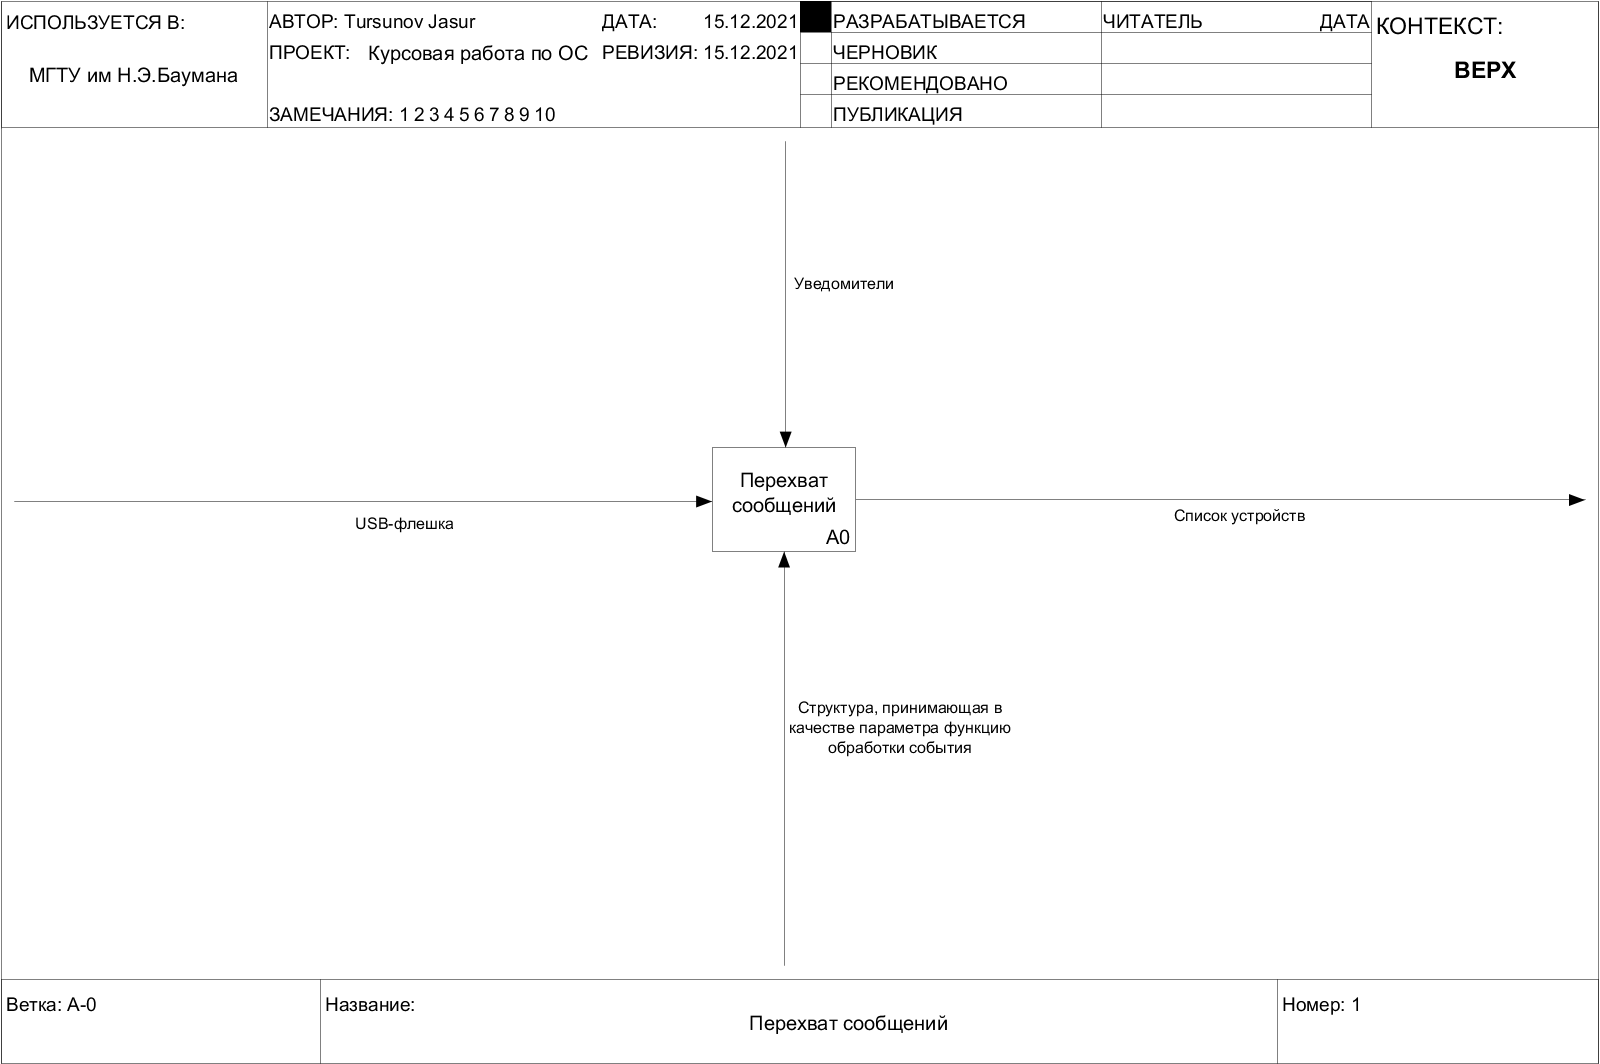
\includegraphics[scale=0.25]{idef0}
			\centering\caption{IDEF0 нулевого уровня}
		\end{figure}
		\begin{figure}[h!]
		\centering
		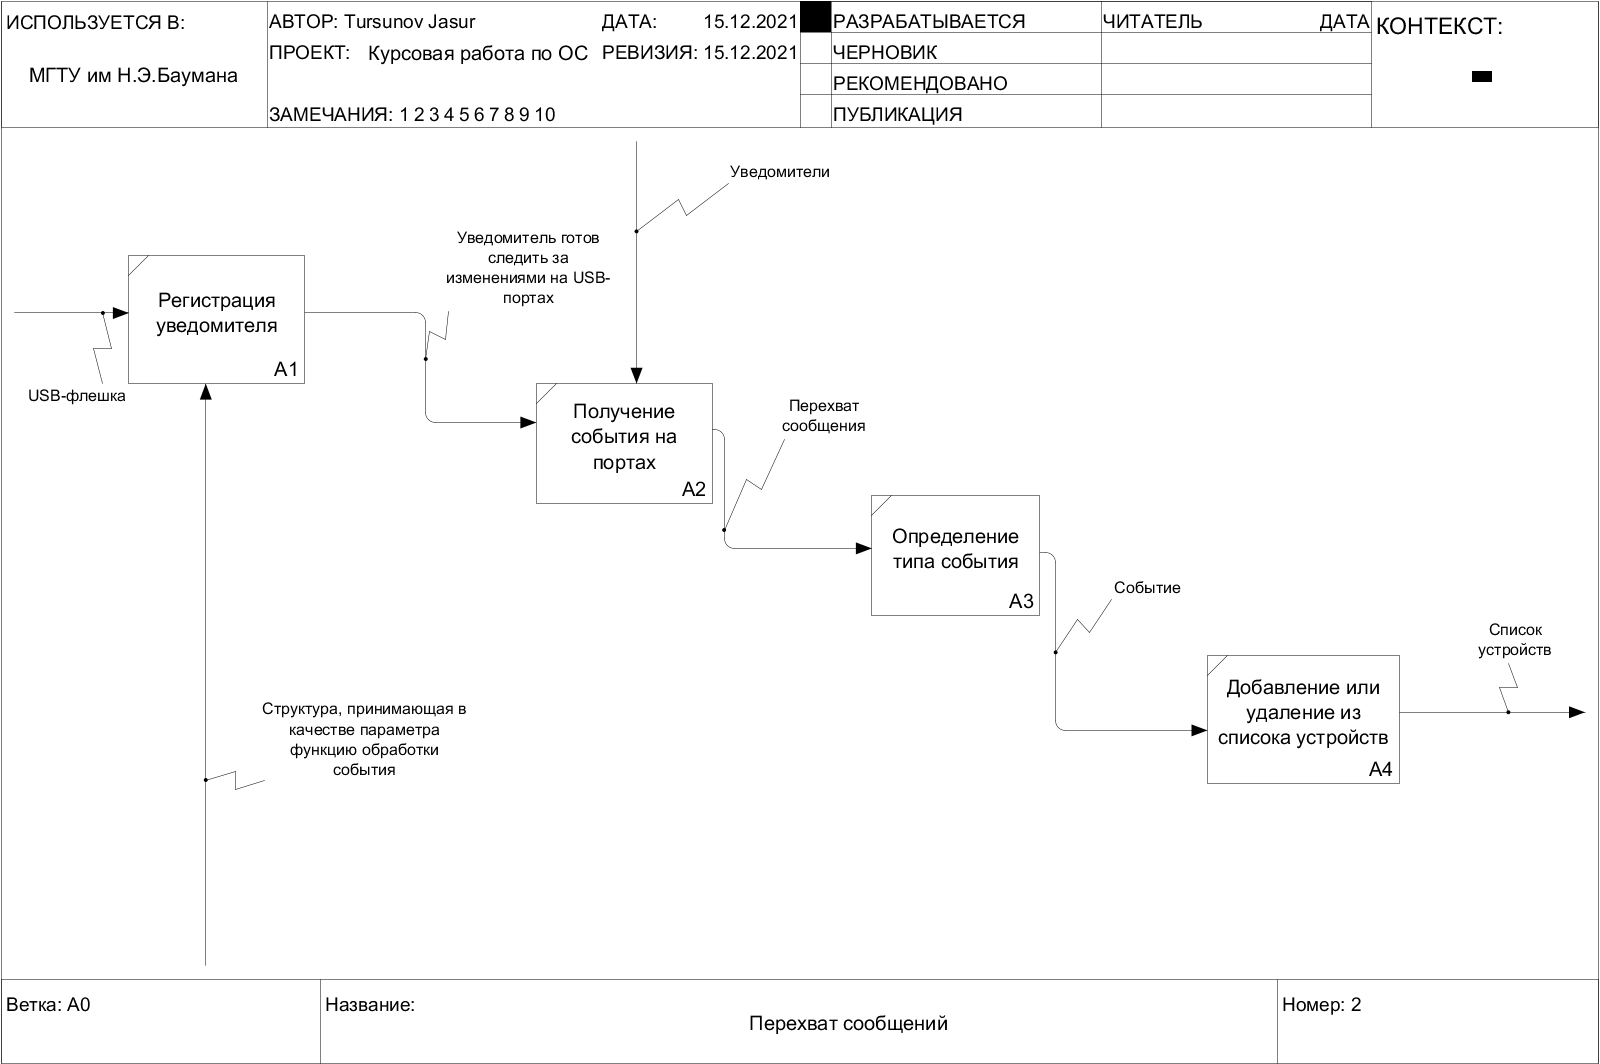
\includegraphics[scale=0.25]{idef1}
		\centering\caption{IDEF0 первого уровня}
	\end{figure}

	Для перехвата сообщений добавление нового USB устройства и удаление USB устройства необходимо в загружаемом модуле ядра разместить уведомитель, принимающий в качества параметра функцию обратного вызова нашей обработки данного события.
	
	Для этого была создана следующая структура представленная в листинге \ref{lst:usb_notify}.
	
	\begin{lstlisting}[language=C, caption = Структура usb\_notify, label=lst:usb_notify]
	static struct notifier_block usb_notify = {
		.notifier_call = notify,
	};
	\end{lstlisting}
	
	В этой структуре содержится указатель на прототип нашей функции обработки:
	
	\hspace*{5mm}\textit{static int notify(struct notifier\_block *self, unsigned long action, void *dev)}
	
	Для создания уведомителя передаем созданную структуру в функцию:
	
	\hspace*{5mm}\textit{usb\_register\_notify(\&usb\_notify);}
	
	Для удаления уведомителя передаем структуру в функцию:
	
	\hspace*{5mm}\textit{usb\_unregister\_notify(\&usb\_notify);}
	\subsection{Хранение информации}
	\hspace*{5mm} Для хранения информации о подключенных USB устройствах создадим структуру, листинг \ref{lst:our_usb_device}.
	
	\begin{lstlisting}[language=C, caption = Структура our\_usb\_device, label =  lst:our_usb_device]
	typedef struct our_usb_device {
		struct usb_device_id dev_id;
		struct list_head list_node;
	} our_usb_device_t;
	\end{lstlisting}
	
	Инициализируем список: \textit{LIST\_HEAD(connected\_devices);}
	
	Для добавления нового подключенного устройства используется функция \ref{lst:add_usb},  для удаления -- \ref{lst:del_usb}.
	\subsection{Алгоритм работы уведомителя}
	На рисунке 3 и 4 представлен алгоритм работы уведомителя, а имеено показана как обрабатываются события доключения и отключения устройств из USB-портов.
	\clearpage
	\newpage
	\begin{figure}[t!]
		\centering
		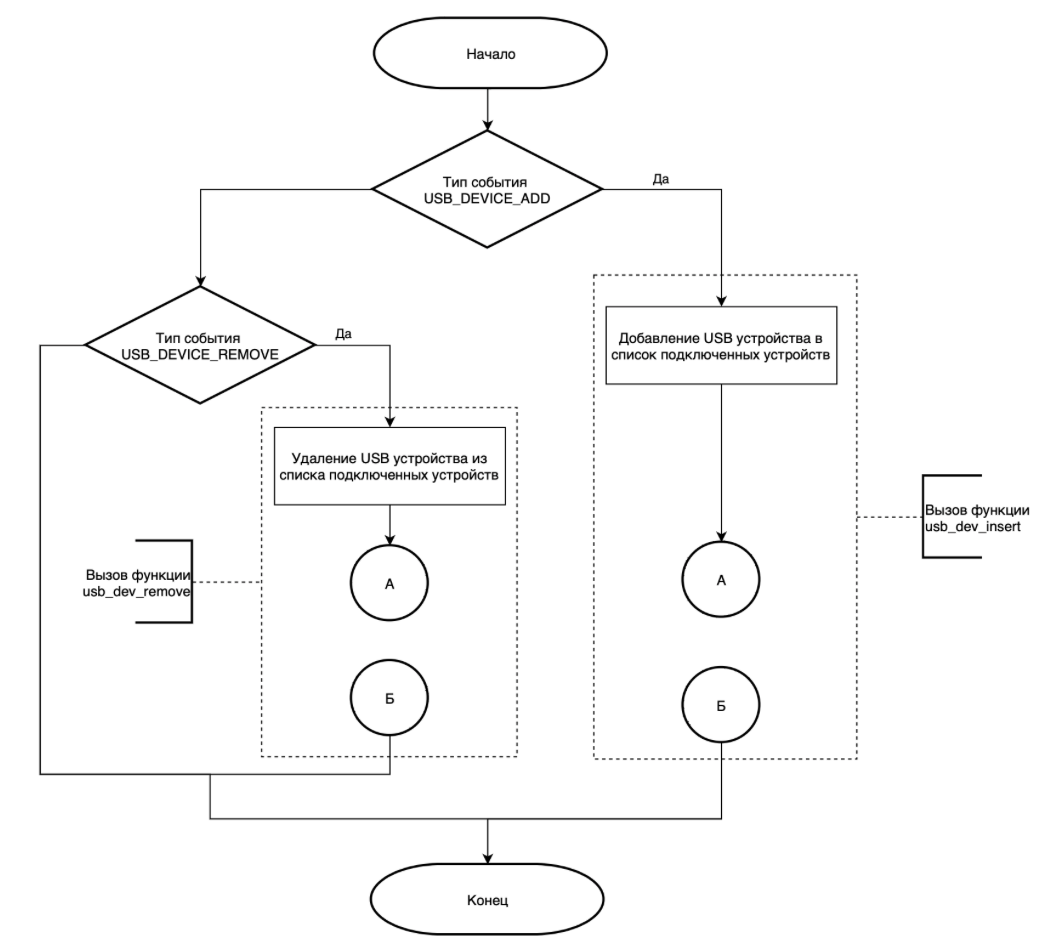
\includegraphics[scale=0.49]{graph1}
		\centering\caption{Алгоритм работы уведомителя.}
	\end{figure}
	\clearpage
	\newpage
	\begin{figure}[t!]
		\centering
		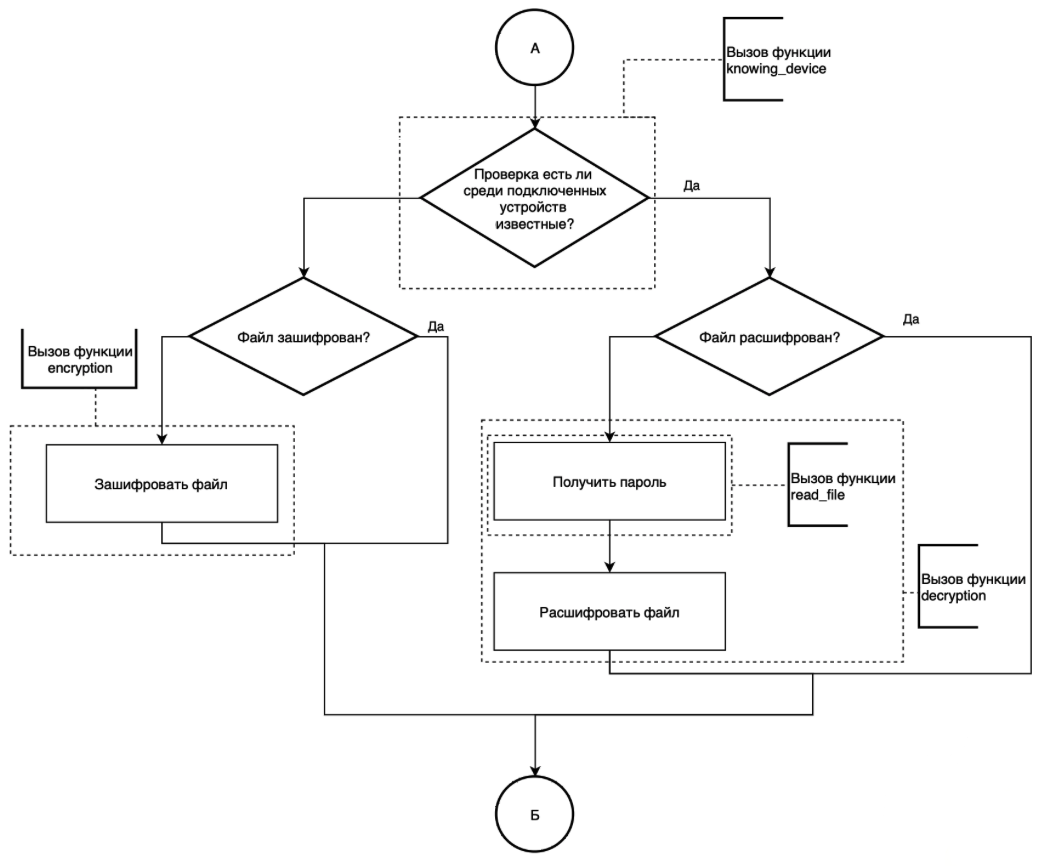
\includegraphics[scale=0.48]{graph2}
		\centering\caption{Алгоритм работы уведомителя.}
	\end{figure}
	\subsection{Алгоритм шифрования файла}
	В качестве алгоритма шифрования был выбран метод шифрования по ключу, блок схема которой представлена на рисунке 5.
	\clearpage
	\newpage
	\begin{figure}[t!]
		\centering
		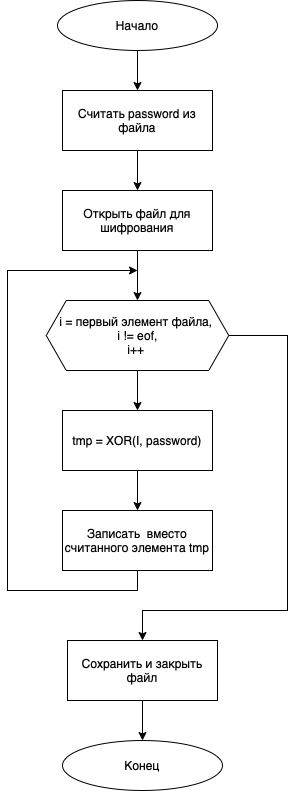
\includegraphics[scale=0.43]{shifr}
		\centering\caption{Алгоритм шифрования по ключу.}
	\end{figure}
	\subsection{Алгоритм определние ключа}
	На рисунке 6 представлена блок-схема плгоритма определения ключа из файла \textit{password.txt} из флешки. 
	\begin{figure}[h!]
		\centering
		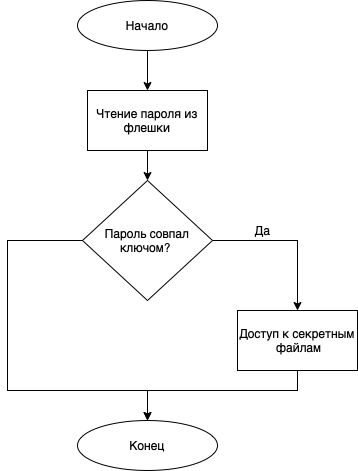
\includegraphics[scale=0.48]{passwoord}
		\centering\caption{Алгоритм определние ключа.}
	\end{figure}
	\subsection{Структура программного обеспечения}
	На рисунке 7 представлена структура разрабатываемого программного обеспечения. Она состоит из двух модулей: создания и удаления.
	\begin{figure}[h!]
		\centering
		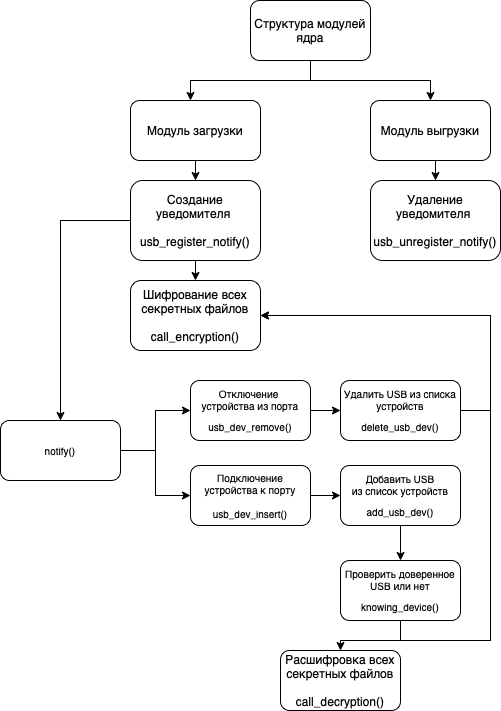
\includegraphics[scale=0.6]{po}
		\centering\caption{Структура программного обеспечения.}
	\end{figure}
\clearpage
\newpage
\section{Технологический раздел}
	\subsection{Выбор языка и среды разработки}
	\hspace*{5mm}Для реализации был выбран язык программирования C. Компилятор -- gcc. Для сборки был написан Makefile, позволяющий запускать сборку, одной командой -- листинг \ref{lst:makefile}. Средой разработки был выбран -- Visual Studio Code.  
	\subsection{Структура хранение данных}
	\hspace*{5mm}Параметры USB устройств, идентификатор поставщика и изделия, а также список секретных файлов и приложений хранятся в конфигурационном файле. Пример конфигурационного файла USB устройств представлен в листинге \ref{lst:config_usb}. Конфигурационный файл секретных файлов и приложений -- листинг \ref{lst:config_file}.
	
	\begin{lstlisting}[language=C,caption = Конфигурационный файл USB устройств, label =  lst:config_usb]
		struct known_usb_device { 
			struct usb_device_id dev_id;    
			char *name;
		};
		
		// List of all USB devices you know
		static const struct known_usb_device known_devices[] = {    
			{ .dev_id = { USB_DEVICE(0x0951, 0x1666) }, 
				.name = "Kingston Technology DataTraveler G4" },
		};
	\end{lstlisting}
	
	\begin{lstlisting}[language=C,caption = Конфигурационный файл секретных файлов и приложений, label =  lst:config_file]  
		static char *secret_apps[] = {    
			"/home/jasur/projects/courseWork-OS/code/file.txt",
			NULL,
		};
	\end{lstlisting}
	
	
	\hspace*{5mm}Пароль для доступа к зашифрованным данным хранится на разрешенном USB устройстве в файле \textit{password.txt}.
	\subsection{Функиция реализующая алгоритм работы уведомителя}
	\hspace*{5mm}В листинге \ref{lst:notify} представлена реализация функции обратного вызова добавления или удаления USB устройства \textit{static int notify(struct notifier\_block *self, unsigned long action, void *dev)}. 
	
	С последующим вызовом, в зависимости от события \textit{static void usb\_dev\_remove(struct usb\_device *dev)}, \textit{static void usb\_dev\_insert(struct usb\_device *dev)}.
	\begin{lstlisting}[language=C,caption = Функция реализующая алгоритм работы уведомителя, label =  lst:notify]
		// If usb device inserted.
		static void usb_dev_insert(struct usb_device *dev)
		{   
			add_our_usb_device(dev);
			char *name = knowing_device();
			
			if (name)
			{
				if (state_encrypt)
				call_decryption(name);
				state_encrypt = false;
				printk(KERN_INFO "USB MODULE: New device we can encrypt.\n");
			}
			else
			{
				if (!state_encrypt)
				call_encryption();
				state_encrypt = true;
				printk(KERN_INFO "USB MODULE: New device, we can't encrypt.\n");
			}
		}
		
		// If usb device removed.
		static void usb_dev_remove(struct usb_device *dev)
		{
			delete_our_usb_device(dev);
			char *name = knowing_device();
			
			if (name)
			{
				if (state_encrypt)
				call_decryption(name);
				state_encrypt = false; 
				printk(KERN_INFO "USB MODULE: Delete device, we can encrypt.\n");
			}
			else
			{
				if (!state_encrypt)
				call_encryption();
				state_encrypt = true;
				printk(KERN_INFO "USB MODULE: Delete device, we can't encrypt.\n");
			}
		}
		
		// New notify.
		static int notify(struct notifier_block *self, unsigned long action, void *dev)
		{
			// Events, which our notifier react.
			switch (action) 
			{
				case USB_DEVICE_ADD:
				usb_dev_insert(dev);
				break;
				case USB_DEVICE_REMOVE:
				usb_dev_remove(dev);
				break;
				default:
				break;
			}
			return 0;
		}
	\end{lstlisting}
	
	\subsection{Функция реализующая алгоритм шифрования}
	\hspace*{5mm}Чтобы узнать можно ли расшифровать файл, необходимо узнать принадлежит ли устройство списку разрешенных устройств. Каждое устройство имеет уникальную пару идентификатор поставщика и идентификатор изделия, по ней и будет происходит поиск. Также в известных устройствах хранится файл с паролем для расшифровки секретных данных.
	
	Реализация данной проверки представлена в листинге \ref{lst:check}.
	\begin{lstlisting}[language=C,caption = Функции для проверки разрешенных устройств, label =  lst:check]
		// Match device id with device id.
		static bool device_id_match_device_id(struct usb_device_id *new_dev_id, 
		const struct usb_device_id *dev_id)
		{
			// Check idVendor and idProduct, which are used.
			if (dev_id->idVendor != new_dev_id->idVendor)
			return false;
			if (dev_id->idProduct != new_dev_id->idProduct)
			return false;
			return true;
		}
		
		// Check our list of devices, if we know device.
		static char *usb_device_id_is_known(struct usb_device_id *dev)
		{
			unsigned long known_devices_len = sizeof(known_devices) / sizeof(known_devices[0]);
			int i = 0;
			for (i = 0; i < known_devices_len; i++)
			{
				if (device_id_match_device_id(dev, &known_devices[i].dev_id))
				{
					int size = sizeof(known_devices[i].name);
					char *name = (char *)kmalloc(size + 1, GFP_KERNEL);
					int j = 0;
					for (j = 0; j < size; j++)
					name[j] = known_devices[i].name[j];
					name[size + 1] = '\0';
					
					return name;
				}
			}
			return NULL;
		}
		
		static char *knowing_device(void)
		{
			our_usb_device_t *temp;
			int count = 0;
			char *name;
			
			list_for_each_entry(temp, &connected_devices, list_node) {
				name = usb_device_id_is_known(&temp->dev_id);
				if (!name)
				return NULL;
				count++;
			}
			if (0 == count)
			return NULL;
			return name;
		}
	\end{lstlisting}
	
	Считывание пароля представлено в листинге \ref{lst:password}.
	
	
	После проверки принадлежности, при необходимости вызываются функции шифровки и расшифровки файлов, которые вызывают исполняемый файл пользовательского пространства.
	
	\begin{lstlisting}[language=C,caption = Считывание пароля из файла USB устройства, label =  lst:password]
		static char *read_file(char *filename)
		{
			struct kstat *stat;
			struct file *fp;
			mm_segment_t fs;
			loff_t pos = 0;
			char *buf;
			int size;
			
			fp = filp_open(filename, O_RDWR, 0644);
			if (IS_ERR(fp))
			{
				return NULL;
			}
			
			fs = get_fs();
			set_fs(KERNEL_DS);
			
			stat = (struct kstat *)kmalloc(sizeof(struct kstat), GFP_KERNEL);
			if (!stat)
			{
				return NULL;
			}
			
			vfs_stat(filename, stat);
			size = stat->size;
			
			buf = kmalloc(size, GFP_KERNEL);
			if (!buf) 
			{
				kfree(stat);
				return NULL;
			}
			
			kernel_read(fp, buf, size, &pos);
			
			filp_close(fp, NULL);
			set_fs(fs);
			kfree(stat);
			buf[size]='\0';
			return buf;
		}
	\end{lstlisting}
	
	Реализация этих функций представлена в листинге \ref{lst:user_call}.
	
\clearpage
\newpage
\section{Исследовательский раздел }
	\subsection{Системные характеристики}
	Характеристики компьютера на котором проводился эксперимент:
	\begin{enumerate}
		\item операционная система - Linux Ubuntu 18.04;
		\item процессор - Intel(R) Core(TM) i7-10510U CPU @1.80GHz 2.30GHz;
		\item объем оперативной памяти - 16 ГБ;
		\item количество ядер - 4;
		\item количество логических процессов - 8;
	\end{enumerate}
	\subsection{Постановка эксперимента}
	В рамках данного проекта были проведены эксперименты, описанные ниже:
	\begin{enumerate}
		\item проверка защищенности секретных файлов при подключение опознанного устройства;
		\item проверка защищенности секретных файлов при подключение неопознанного устройства;
		\item Корректная обработка в случае, если подключено разрешенное и неразрешенное устройства одновременно.
	\end{enumerate}
	\subsection{Пример работы}
	\hspace*{5mm}На рисунке 3 показан пример успешной загрузки полученного модуля в ядро/ Секретный файл <<file.txt>> -- зашифрован.
	\begin{figure}[h!]
		\centering
		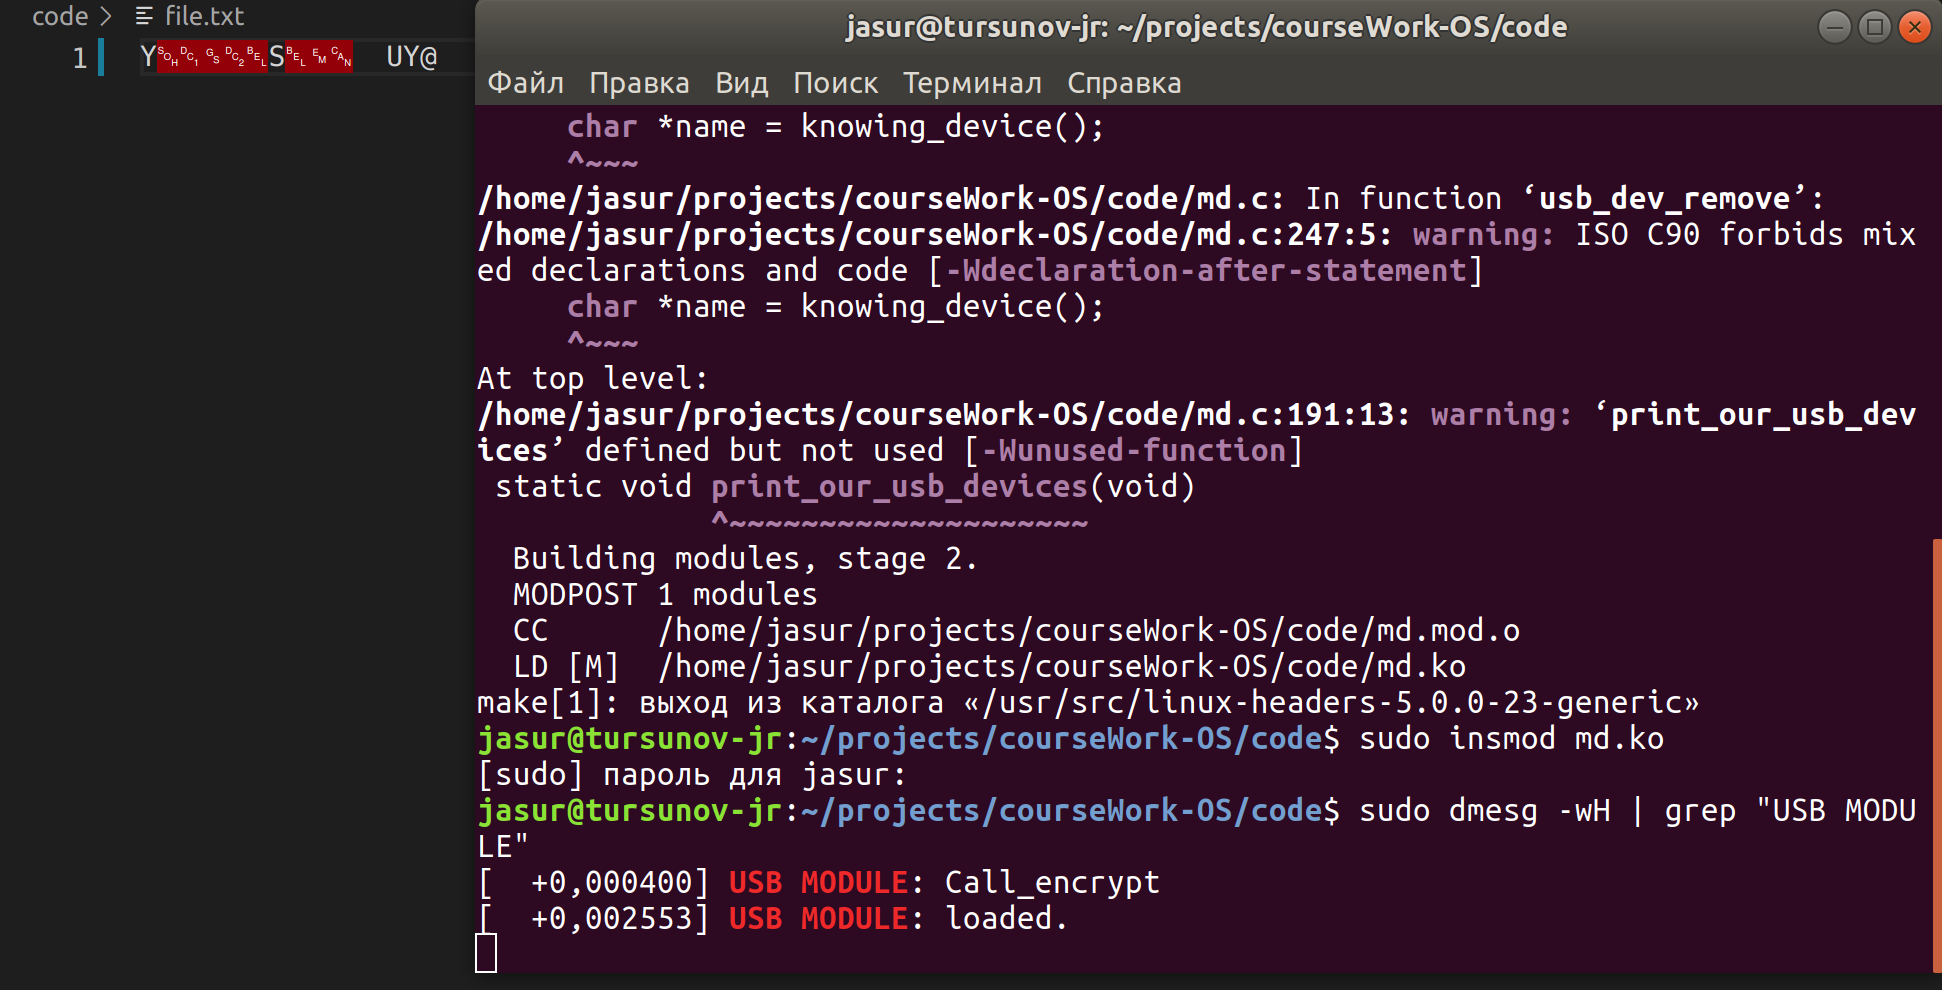
\includegraphics[scale=0.2]{1}
		\centering\caption{Успешная загрузка модуля в ядро.}
	\end{figure}
	\clearpage
	\newpage
	На рисунке 4 показан расшифрованный секретный файл, так как было подключение доверенного USB-устройства.
	\begin{figure}[h!]
		\centering
		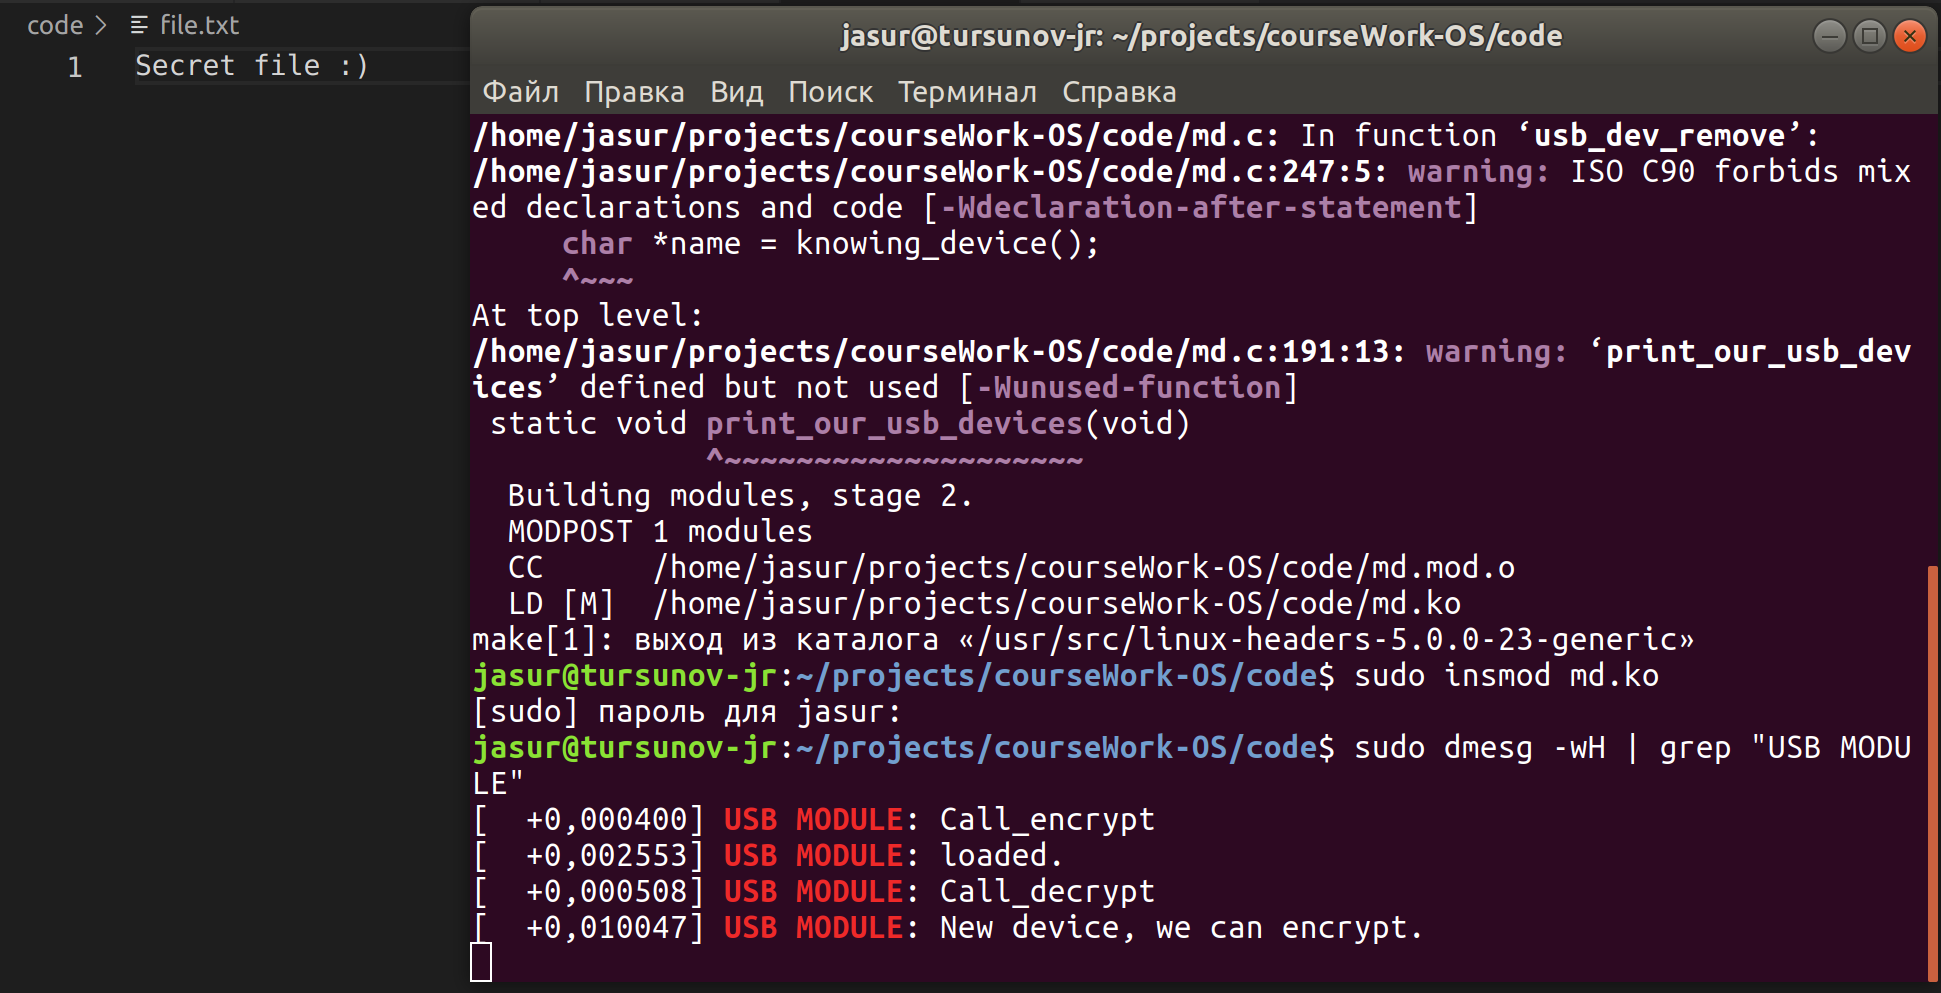
\includegraphics[scale=0.2]{2}
		\centering\caption{Подключение доверенного USB-устройства.}
	\end{figure}
	\\ \hspace*{5mm} На рисунке 5 показан случай, когда происходит отключение доверенного USB-устройства, при этом отсутствуют иные устройства на портах компьютера.
	\begin{figure}[h!]
		\centering
		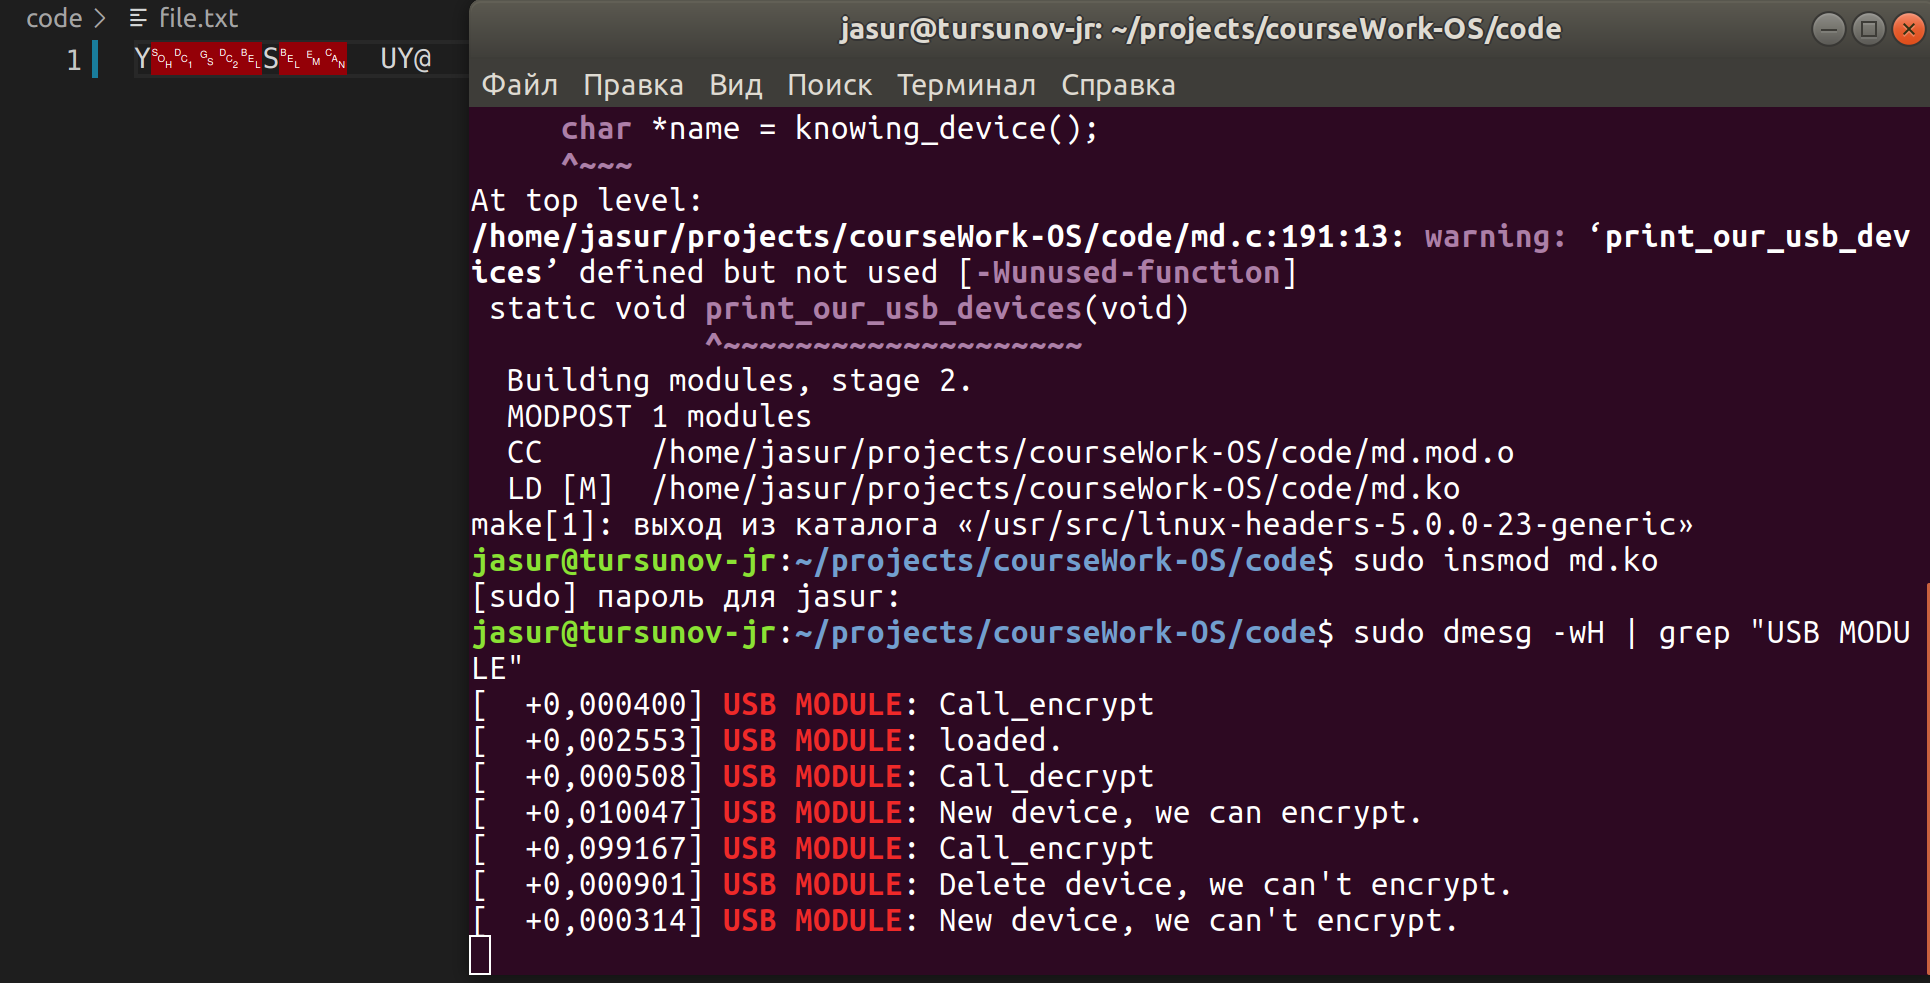
\includegraphics[scale=0.2]{3}
		\centering\caption{Отключение доверенного USB-устройства.}
	\end{figure}
	\\ \hspace*{5mm} Рисунок 6 показывает поведение системы, когда подклено неопознанное USB-устройство. Секретный файл -- зашифрован и не доступен для использования.
	\clearpage
	\newpage
	\begin{figure}[h!]
		\centering
		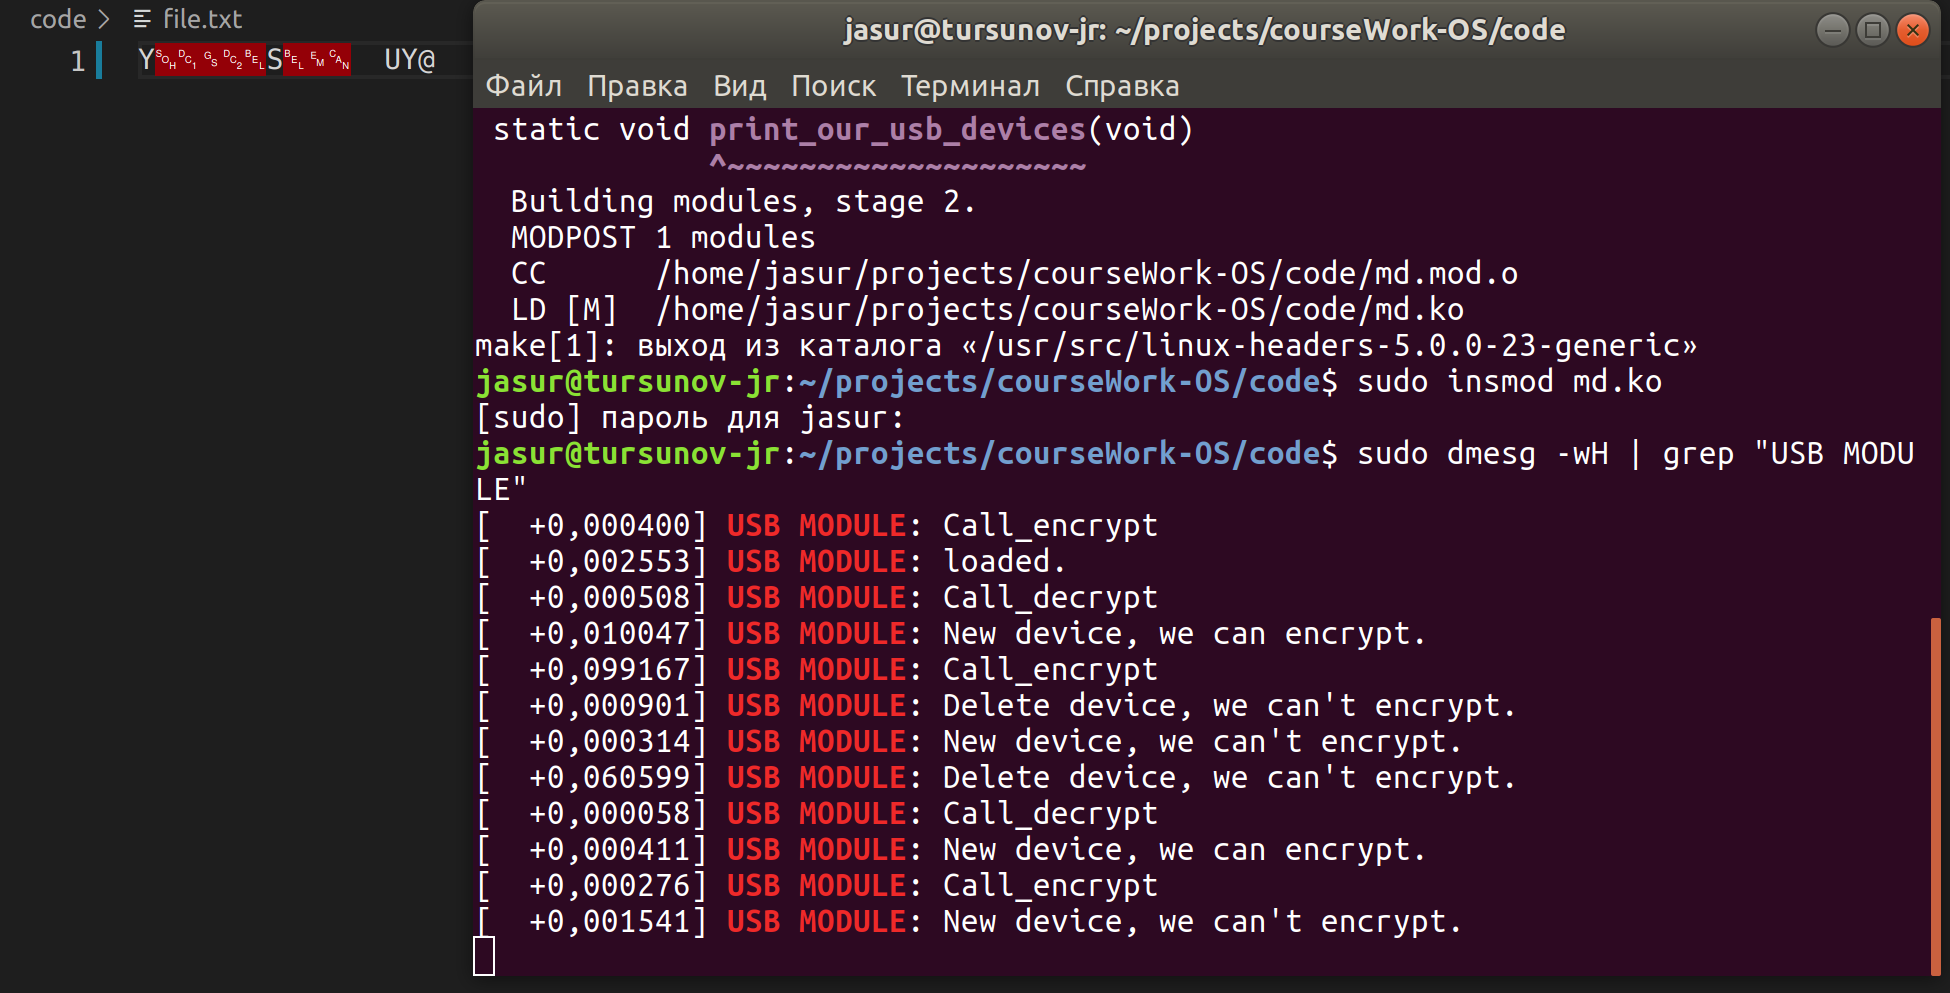
\includegraphics[scale=0.2]{4}
		\centering\caption{Подключение неопознанного USB-устройства.}
	\end{figure}
	\hspace*{5mm} На рисунке 7 представлен случай, когда подключено одновременно два устройства: доверенное и нет. Как видно на рисунке секретный файл сохранил свою ценность, так как остался зашифрованным. В конце можно заметить, что произошла успешная выгрузка модуля из ядра -- функционал перестал работать. 
	\begin{figure}[h!]
		\centering
		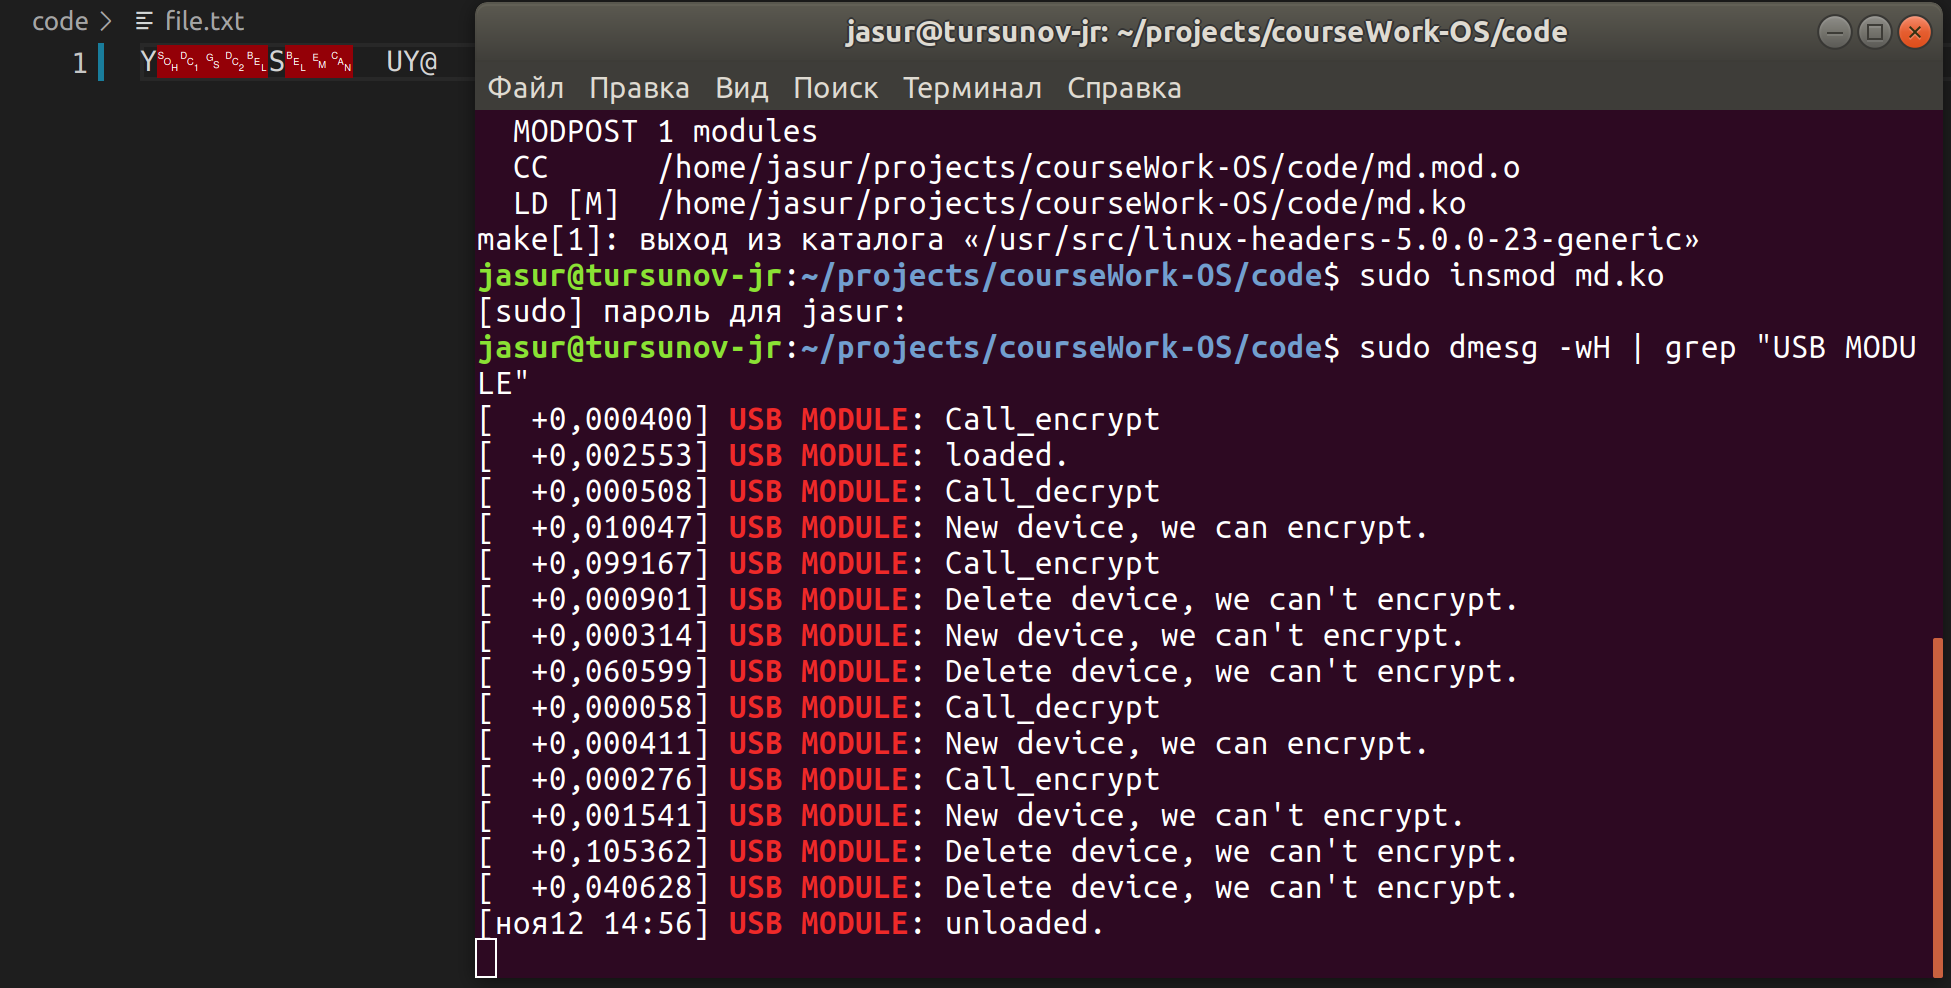
\includegraphics[scale=0.2]{5}
		\centering\caption{Одновременное подключение опознанного и неопознанного USB-устройства.}
	\end{figure}
	\clearpage
	\newpage
\section*{Заключение}
	\addcontentsline{toc}{section}{Заключение}
	В результате курсовой работы по операционной системе:
	\begin{enumerate}
		\item[1. ] проанализированы способы защиты при помощи USB флеш-памяти;
		\item[2. ] разработаны алгоритмы работы функции-обработчика и шифрования файлов;
		\item[3. ] реализован загружаемый модуль ядра.
	\end{enumerate}
	
	Достигнута цель работы -- реализация загружаемого модуля для защиты персональных данных. 
\clearpage
\newpage

\section*{Список литературы}
\addcontentsline{toc}{section}{Список литературы}
[1] \hspace{2mm} Утечки данных 2019: статистика // https://vc.ru/services/103616-utechki-dannyh-2019-statistika-tendencii-kiberbezopasnosti-i-mery-po-snizheniyu-riskov-vzloma (дата обращения: 14.10.2021).\vspace{3mm}
\newline [2]\hspace{2mm} Анатомия загружаемых модулей ядра Linux // https://www.ibm.com/developerworks/ru/library/l-lkm/index.html" (дата обращения: 15.10.2021).\vspace{3mm}
\newline [3]\hspace{2mm} Notification Chains in Linux Kernel// https://0xax.gitbooks.io/linux-insides/content/Concepts/linux-cpu-4.html (дата обращения: 25.10.2021)\vspace{3mm} 
\newline [4]\hspace{2mm} include/linux/usb.h// https://elixir.bootlin.com/linux/latest/source/include/linux/usb.hL2020(дата обращения: 03.11.2021).\vspace{3mm}
\newline [5]\hspace{2mm} Doubly Linked Lists // https://www.kernel.org/doc/html/v4.14/core-api/kernel-api.html (дата обращения: 03.11.2021).\vspace{3mm}
\newline [6]\hspace{2mm} Invoking user-space applications from the kernel // https://developer.ibm.com/technologies/linux/articles/l-user-space-apps/ (дата обращения: 04.11.2021).\vspace{3mm}
\newline [7]\hspace{2mm} Reading and writing of files in Linux kernel driver // https://www.programmersought.com/article/83015124510/ (дата обращения: 04.11.2021).\vspace{3mm}

\clearpage
\newpage

\section*{Листинг}
\addcontentsline{toc}{section}{Листинг}
\begin{lstlisting}[language=C, caption = Структура usb\_device, label =  lst:usb_device]
	struct usb_device {
		int		devnum;
		char		devpath[16];
		u32		route;
		enum usb_device_state	state;
		enum usb_device_speed	speed;
		unsigned int		rx_lanes;
		unsigned int		tx_lanes;
		
		struct usb_tt	*tt;
		int		ttport;
		
		unsigned int toggle[2];
		
		struct usb_device *parent;
		struct usb_bus *bus;
		struct usb_host_endpoint ep0;
		
		struct device dev;
		
		struct usb_device_descriptor descriptor;
		struct usb_host_bos *bos;
		struct usb_host_config *config;
		
		struct usb_host_config *actconfig;
		struct usb_host_endpoint *ep_in[16];
		struct usb_host_endpoint *ep_out[16];
		
		char **rawdescriptors;
		
		unsigned short bus_mA;
		u8 portnum;
		u8 level;
		u8 devaddr;
		
		unsigned can_submit:1;
		unsigned persist_enabled:1;
		unsigned have_langid:1;
		unsigned authorized:1;
		unsigned authenticated:1;
		unsigned wusb:1;
		unsigned lpm_capable:1;
		unsigned usb2_hw_lpm_capable:1;
		unsigned usb2_hw_lpm_besl_capable:1;
		unsigned usb2_hw_lpm_enabled:1;
		unsigned usb2_hw_lpm_allowed:1;
		unsigned usb3_lpm_u1_enabled:1;
		unsigned usb3_lpm_u2_enabled:1;
		int string_langid;
		
		/* static strings from the device */
		char *product;
		char *manufacturer;
		char *serial;
		
		struct list_head filelist;
		
		int maxchild;
		
		u32 quirks;
		atomic_t urbnum;
		
		unsigned long active_duration;
		
		#ifdef CONFIG_PM
		unsigned long connect_time;
		
		unsigned do_remote_wakeup:1;
		unsigned reset_resume:1;
		unsigned port_is_suspended:1;
		#endif
		struct wusb_dev *wusb_dev;
		int slot_id;
		enum usb_device_removable removable;
		struct usb2_lpm_parameters l1_params;
		struct usb3_lpm_parameters u1_params;
		struct usb3_lpm_parameters u2_params;
		unsigned lpm_disable_count;
		
		u16 hub_delay;
		unsigned use_generic_driver:1;
	};
\end{lstlisting}

\begin{lstlisting}[language=C, caption = Структура usb\_device\_id, label =  lst:usb_device_id]
	struct usb_device_id {
		/* which fields to match against? */
		__u16		match_flags;
		
		/* Used for product specific matches; range is inclusive */
		__u16		idVendor;
		__u16		idProduct;
		__u16		bcdDevice_lo;
		__u16		bcdDevice_hi;
		
		/* Used for device class matches */
		__u8		bDeviceClass;
		__u8		bDeviceSubClass;
		__u8		bDeviceProtocol;
		
		/* Used for interface class matches */
		__u8		bInterfaceClass;
		__u8		bInterfaceSubClass;
		__u8		bInterfaceProtocol;
		
		/* Used for vendor-specific interface matches */
		__u8		bInterfaceNumber;
		
		/* not matched against */
		kernel_ulong_t	driver_info
		__attribute__((aligned(sizeof(kernel_ulong_t))));
	};
\end{lstlisting}

\begin{lstlisting}[language=C, caption = Добавление usb устройства, label =  lst:add_usb]
	static void add_our_usb_device(struct usb_device *dev)
	{
		our_usb_device_t* new_usb_device = (our_usb_device_t *)kmalloc
		(sizeof(our_usb_device_t), GFP_KERNEL);
		struct usb_device_id new_id = { USB_DEVICE(dev->descriptor.idVendor, 
			dev->descriptor.idProduct) };
		new_usb_device->dev_id = new_id;
		list_add_tail(&new_usb_device->list_node, &connected_devices);
	}
\end{lstlisting}

\begin{lstlisting}[language=C, caption = Удаление usb устройства, label =  lst:del_usb]
	static void delete_our_usb_device(struct usb_device *dev)
	{
		our_usb_device_t *device, *temp;
		list_for_each_entry_safe(device, temp, &connected_devices, list_node) 
		{
			if (device_match_device_id(dev, &device->dev_id))
			{
				list_del(&device->list_node);
				kfree(device);
			}
		}
	}
\end{lstlisting}

\begin{lstlisting}[language=C, caption = Makefile, label =  lst:makefile]
	ifneq ($(KERNELRELEASE),)
	obj-m := md.o
	else
	CURRENT = $(shell uname -r)
	KDIR = /lib/modules/$(CURRENT)/build
	PWD = $(shell pwd)
	
	default:
	$(MAKE) -C $(KDIR) M=$(PWD) modules
	
	clean:
	rm -rf .tmp_versions
	rm *.ko
	rm *.o
	rm *.mod.c
	rm *.symvers
	rm *.order
	
	endif
\end{lstlisting}

\begin{lstlisting}[language=C,caption = Загрузка и удаление модуля ядра, label =  lst:module]
	static int __init my_module_init(void)
	{
		usb_register_notify(&usb_notify);
		call_encryption();
		printk(KERN_INFO "USB MODULE: loaded.\n");
		return 0;
	}
	
	static void __exit my_module_exit(void)
	{
		usb_unregister_notify(&usb_notify);    
		printk(KERN_INFO "USB MODULE: unloaded.\n");
	}
	
	module_init(my_module_init);
	module_exit(my_module_exit);
\end{lstlisting}






\begin{lstlisting}[language=C,caption = Функции вызывающие исполняемый файл пользовательского пространства, label =  lst:user_call]
	static int call_decryption(char *name_device) {
		printk(KERN_INFO "USB MODULE: Call_decrypt\n");
		
		char path[80];
		strcpy(path, USB_FOLDER);
		strcat(path, name_device);
		strcat(path, "/");
		strcat(path, PASSWORD_FILE);
		char *data = read_file(path);
		
		char *argv[] = {
			"/home/jasur/projects/courseWork-OS/code/crypto",
			data,
			NULL };
		
		static char *envp[] = {
			"HOME=/",
			"TERM=linux",
			"PATH=/sbin:/bin:/usr/sbin:/usr/bin", 
			NULL };
		
		if (call_usermodehelper(argv[0], argv, envp, UMH_WAIT_PROC) < 0) 
		{
			return -1;
		}
		
		return 0;
	}
	
	static int call_encryption(void) {
		printk(KERN_INFO "USB MODULE: Call_encrypt\n");
		char *argv[] = {
			"/home/jasur/projects/courseWork-OS/code/crypto",
			NULL };
		
		static char *envp[] = {
			"HOME=/",
			"TERM=linux",
			"PATH=/sbin:/bin:/usr/sbin:/usr/bin", 
			NULL };
		
		if (call_usermodehelper(argv[0], argv, envp, UMH_WAIT_PROC) < 0) 
		{
			return -1;
		}
		
		return 0;
	}
\end{lstlisting}
\end{document}